% Section 1: Setting up the environment
\newpage
\section{Nastavení prostředí}
Běžné programování v Pythonu silně spoléhá na externí balíčky, které mohou mít různé verze a závislosti. Aby se předešlo konfliktům mezi různými projekty, doporučuje se pro každý projekt používat virtuální prostředí (\emph{virtual environment}, alebo ve zkratce venv). V tomto kurzu budeme takové virtuální prostředí používat, abychom zajistili konzistentní vývojové prostředí pro všechny. Virtuální prostředí jsou doporučeným způsobem správy závislostí v projektech v Pythonu.

Pro správu těchto virtuálních prostředí budeme používat open-source nástroj \verb|uv|, dostupný na \url{https://github.com/astral-sh/uv}. Pokud již máte nainstalovanou jakoukoli verzi Pythonu, můžete \verb|uv| nainstalovat jednoduchým spuštěním
\begin{lstlisting}
pip install uv
\end{lstlisting}
Pokud Python nainstalovaný nemáte, můžete si jej stáhnout z \url{https://www.python.org/downloads/} a poté použít výše uvedený příkaz nebo použít samostatné instalátory na \url{https://github.com/astral-sh/uv}.

Pro otestování instalace spusťte v příkazovém řádku
\begin{lstlisting}
uv --version
\end{lstlisting}
a mělo by se objevit něco podobného jako \verb|uv 0.5.30|.

Nyní vytvoříme projekt s názvem \verb|NOFY080_2025|, který bude obsahovat všechny soubory související s tímto kurzem, spuštěním
\begin{lstlisting}
uv init NOFY080_2025
\end{lstlisting}
který vytvoří nový adresář se stejným názvem, s jednoduchým souborem "Hello World" v Pythonu, několika dalšími soubory, které \verb|uv| používá ke sledování závislostí vašeho projektu, a nastaví v něm git repozitář (v tomto kurzu nemusíte používat git, ale zájemci se mohou naučit základy v dodatku~\ref{sec:git}).

Nyní se přesuňte do adresáře projektu
\begin{lstlisting}
cd NOFY080_2025
\end{lstlisting}
a přidejte balíčky, které budeme v průběhu tohoto kurzu potřebovat
\begin{lstlisting}
uv add numpy scipy matplotlib
\end{lstlisting}
což vytvoří virtuální prostředí a nainstaluje zadané balíčky (v adresáři projektu by se měl objevit adresář \verb|.venv|).

Pokud byste chtěli vytvořit virtuální prostředí bez instalace jakýchkoli balíčků, mohli byste použít příkaz
\begin{lstlisting}
uv venv <name of the virtual environment>
\end{lstlisting}

Pro aktivaci virtuálního prostředí spusťte následující příkaz v Linuxu nebo Mac OS
\begin{lstlisting}
source .venv\bin\activate
\end{lstlisting}
a ve Windows
\begin{lstlisting}
.venv\Scripts\activate
\end{lstlisting}

Nyní, když spustíte \verb|python|, spustí se verze z virtuálního prostředí, nikoli vaše systémová verze. Pro deaktivaci virtuálního prostředí jednoduše spusťte \verb|deactivate|.

\subsection{Spouštění kódu v Pythonu}
Python je interpretovaný jazyk, který není třeba před spuštěním kompilovat. Kód v Pythonu ukládáme do textových souborů s příponou \verb|.py| nebo do takzvaných Jupyter notebooků (přípona souboru \verb|.ipynb|).

Pro otestování naší instalace vytvořte v našem projektovém adresáři nový soubor Pythonu (textový soubor s příponou \verb|.py|) \verb|test.py| s následujícím obsahem
\begin{lstlisting}
import matplotlib.pyplot as plt

plt.plot([1, 2, 3], [4, 5, 6], '-o')
plt.show()
\end{lstlisting}
Pro jeho spuštění můžete buď manuálně aktivovat virtuální prostředí a spustit jej pomocí\\
\verb|python test.py| nebo použít \verb|uv run test.py|. Měl by se objevit jednoduchý graf. Ve zbytku těchto skript myslíme příkazem \verb|python| ten, který spouštíme z virtuálního prostředí .

Pro spuštění kódu v Pythonu přímo, bez uložení do souboru, otevřete vhodný terminál a zadejte \verb|python| - objeví se výzva (\emph{prompt})
\begin{lstlisting}
    >>>
\end{lstlisting}
Toto je Read-Evaluate-Print-Loop (REPL); jakýkoli zadaný kód bude spuštěn a výsledek vytištěn na obrazovku. Pro ukončení zadejte \verb|quit()|. Pro spuštění souboru \verb|myfile.py| se nejprve přesuňte do jeho adresáře a poté jej jednoduše spusťte pomocí \verb|python myfile.py| (všimněte si, že pokud máte aktivované virtuální prostředí, skutečný skript Pythonu se nemusí nacházet ve vašem projektovém adresáři).

\begin{exercise}
    Vytvořte textový soubor \verb|hello.py|, který obsahuje jeden řádek
    \begin{lstlisting}
        print("Hello world!")
    \end{lstlisting}
    a poté tento soubor spusťte.
\end{exercise}

Někdy nechceme, aby se interpreter Pythonu ukončil ihned po dokončení běhu našeho programu (např. chceme zkontrolovat proměnné vytvořené během běhu programu); to lze provést pomocí\\ \verb|python -i file.py|, kde \verb|-i| znamená \emph{interaktivní}. Alternativně lze uživatelsky přívětivější (barevně odlišená syntaxe, automatické doplňování atd.) verzi interaktivního Python REPL vyvolat pomocí \verb|ipython| (nebo \verb|ipython3|, v závislosti na vaší instalaci), který lze také použít k interaktivnímu spouštění souborů pomocí \verb|ipython3 -i myfile.py|.

\subsection{Krátká poznámka k textovým editorům}
K psaní kódu v Pythonu lze použít jakýkoli textový editor, včetně výchozího Poznámkového bloku ve Windows. Pro vaše duševní zdraví je však přínosné používat alespoň něco se zvýrazňováním syntaxe, jako je Notepad++, nebo editor s více funkcemi, jako je VS Code nebo Spyder, kde můžete soubor spustit bez přepínání do terminálu. V tomto kurzu doporučuji používat VS Code s nainstalovaným rozšířením pro Python, protože usnadňuje práci s virtuálními prostředími. Při otevření adresáře VS Code automaticky detekuje virtuální prostředí a použije ho při spuštění souboru. Název aktuálně používaného virtuálního prostředí je uveden v pravém dolním rohu (zvýrazněno červeně):
\begin{center}
    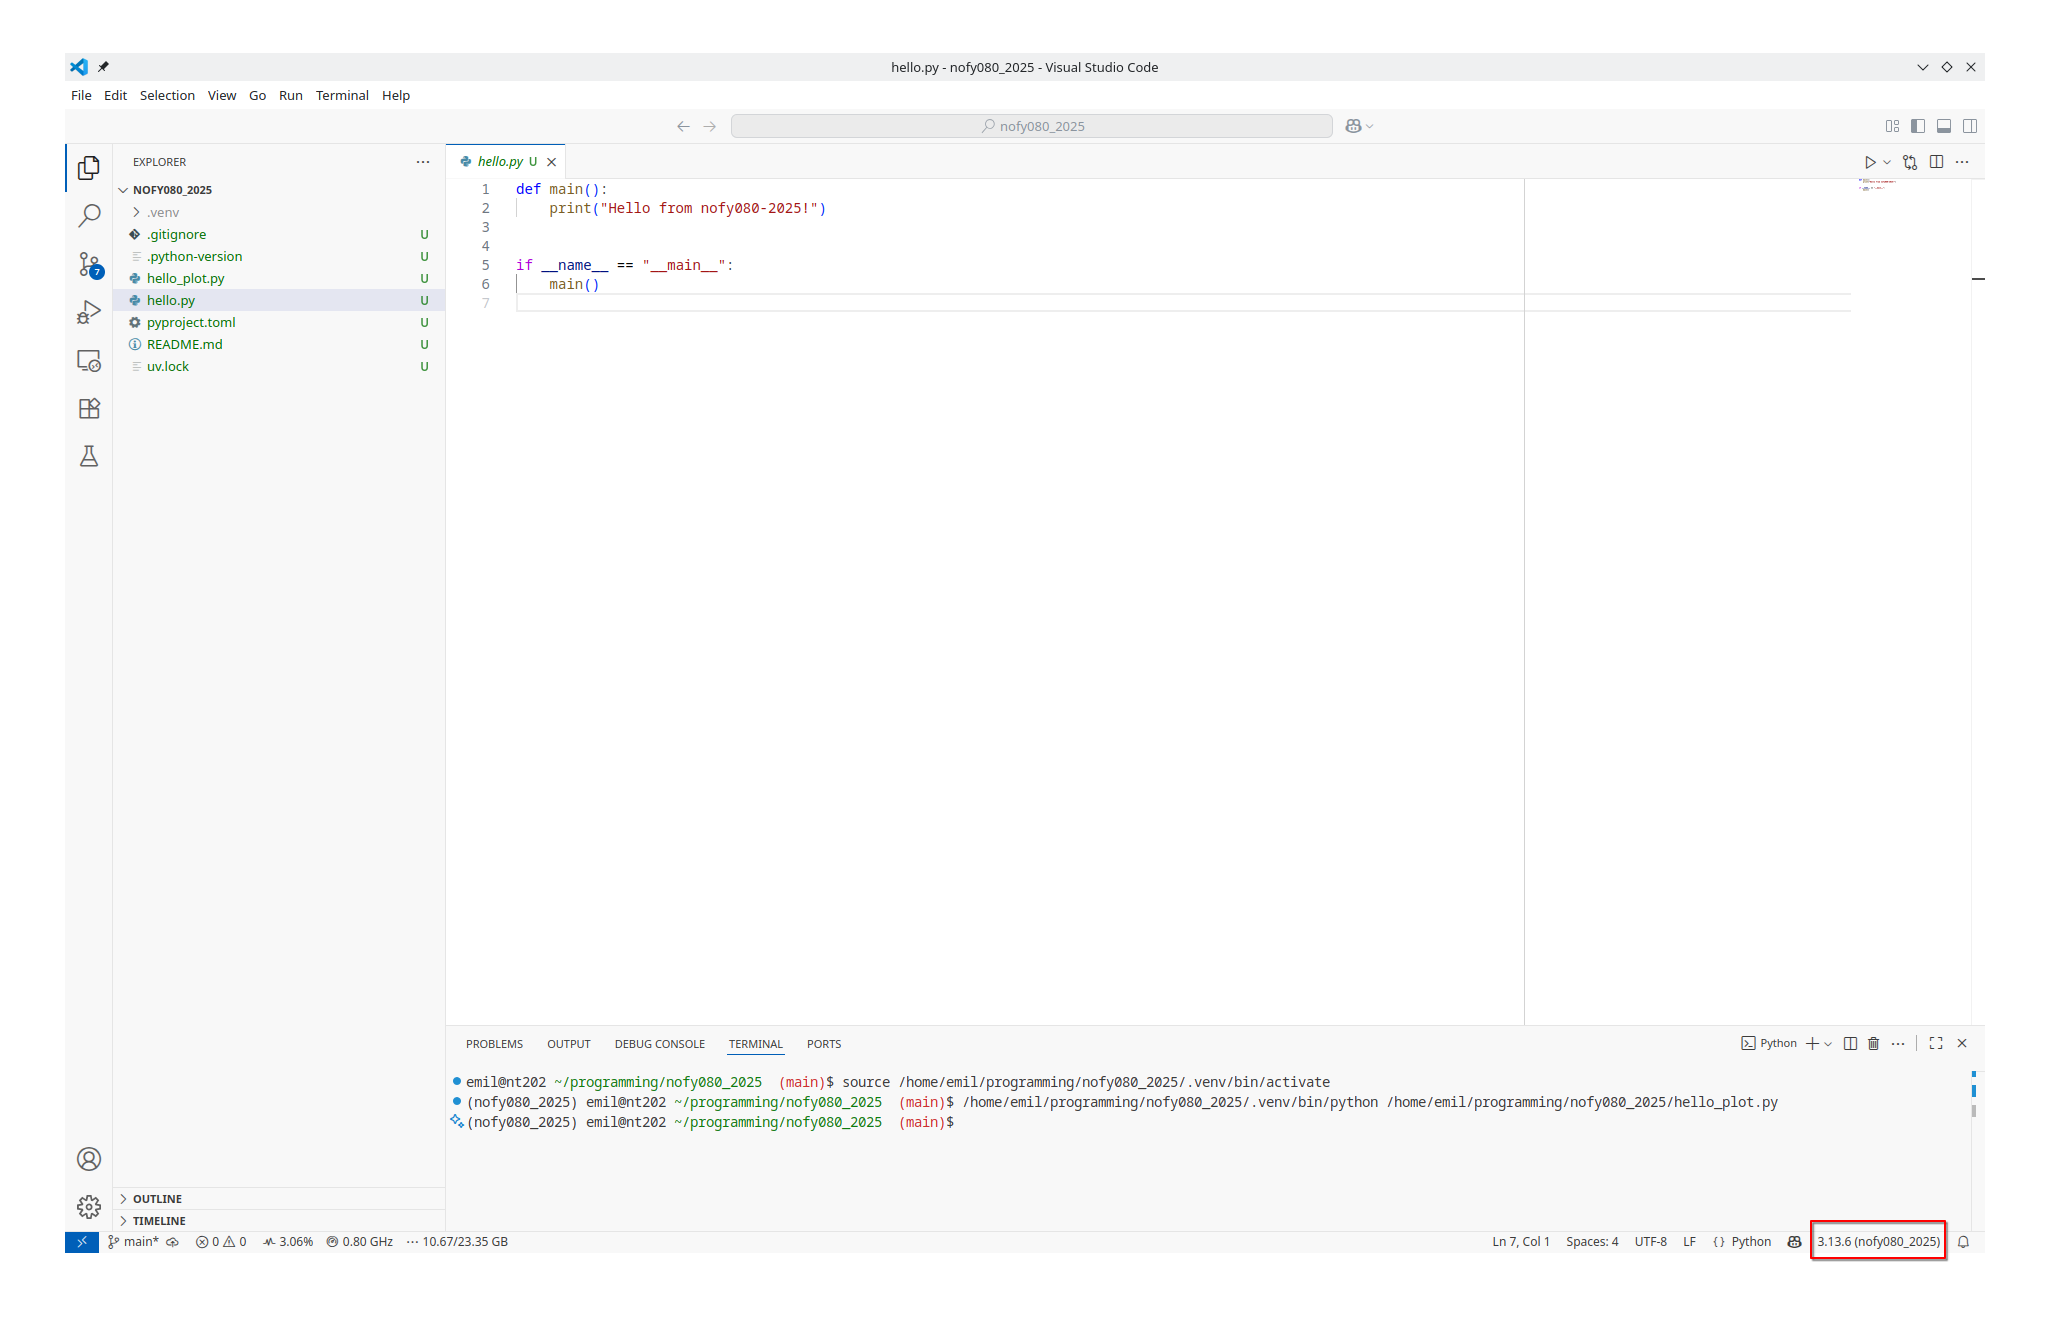
\includegraphics[width=0.9\linewidth]{vscode.png}
\end{center}

Práce s prostředími ve Spyderu je poněkud složitější; viz průvodce \href{https://github.com/spyder-ide/spyder/wiki/Working-with-packages-and-environments-in-Spyder#working-with-other-environments-and-python-installations}{zde}.

\subsubsection{Jupyter Notebooky}
Jupyter notebooky (spouštěné pomocí \verb|jupyter-notebook| v příkazovém řádku) poskytují snadno použitelné interaktivní prostředí s rozhraním běžícím ve webovém prohlížeči, a jsou dobré pro jednoduché vyzkoušení kódu\footnote{V tomto kurzu budeme (většinou) používat skripty kvůli snazšímu rozdělení do modulů a menšímu počtu problémů s paralelním programováním, se kterými se setkáme později.}. Jupyter notebooky také dobře fungují s virtuálními prostředími a VS Code. Přejděte do adresáře svého projektu a spusťte
\begin{lstlisting}
uv pip install jupyter ipympl
\end{lstlisting}
Balíček \verb|ipympl| umožňuje použití interaktivních grafů Matplotlib v Jupyter noteboocích. Dále si také nainstalujte rozšíření \verb|jupyter| ve VS Code. Nyní jednoduše vytvořte soubor s příponou \verb|.ipynb| a můžete jej používat ve VS Code stejně jako v prohlížeči. Při prvním spuštění budete požádáni o výběr virtuálního prostředí, ve kterém by měl notebook běžet; to, které jsme vytvořili, by mělo být jednou z možností, pokud je notebook uložen v projektovém adresáři (stejný adresář jako adresář \verb|.venv|).

\begin{center}
    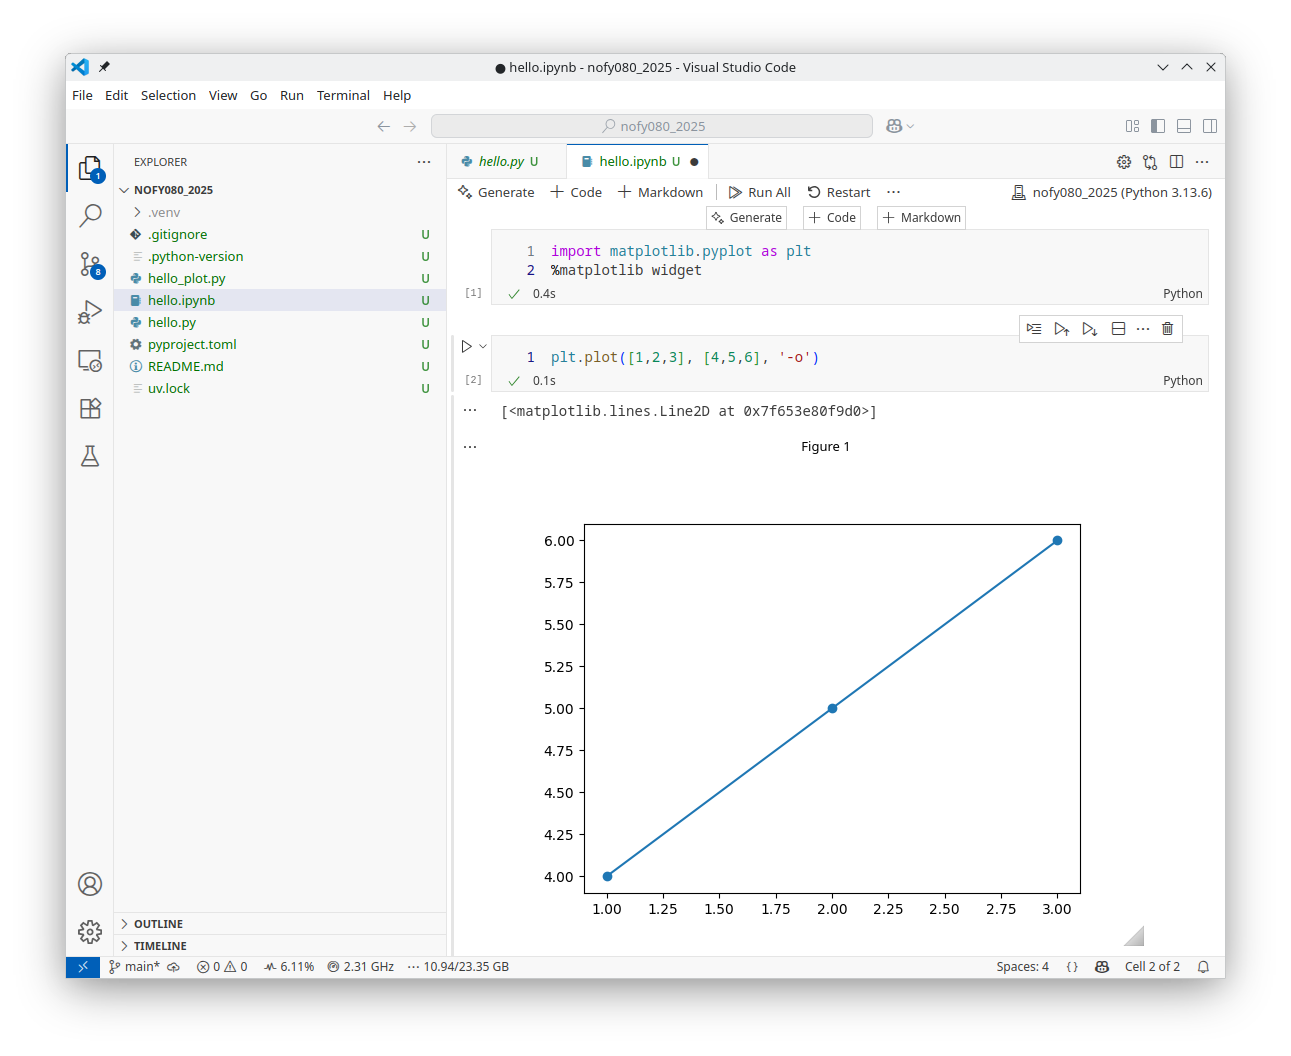
\includegraphics[width=0.9\linewidth]{vscode_jupyter.png}
\end{center}